\documentclass[aspectratio=169]{beamer}
\usepackage[utf8]{inputenc}
\usepackage{fontspec}
\usepackage{booktabs}
\usepackage{listings}
\usepackage{xcolor}
\usepackage{graphicx}
\usepackage{caption}

\usetheme{Madrid}
\usecolortheme{default}

% Configure listings for Python
\lstset{
    language=Python,
    basicstyle=\ttfamily\footnotesize,
    keywordstyle=\color{blue}\bfseries,
    stringstyle=\color{red},
    commentstyle=\color{green!60!black},
    numbers=left,
    numberstyle=\tiny\color{gray},
    stepnumber=1,
    frame=single,
    breaklines=true,
    breakatwhitespace=true,
    showstringspaces=false,
    tabsize=4,
    captionpos=b
}

\title[Chương 12]{Chương 12: Mô hình tùy chỉnh và Huấn luyện với TensorFlow}
\author{Giảng viên: TS. Trần Thành Thắng}
\institute{Đại học Đông Á}
\date{Năm học 2024-2025}

\begin{document}

\begin{frame}
    \titlepage
\end{frame}

\begin{frame}{Nội dung chương}
    \tableofcontents
\end{frame}

\section{Giới thiệu TensorFlow \& Kiến trúc}

\begin{frame}{Giới thiệu nhanh về TensorFlow}
    \begin{itemize}
        \item TensorFlow là thư viện tính toán số học mãnh mẽ mã nguồn mở, đặc biệt phù hợp cho học máy quy mô lớn và học sâu.
        \item Cốt lõi của nó tương tự NumPy, nhưng thao tác với \textbf{Tensor} thay vì mảng.
        \item Cung cấp khả năng tính toán vượt trội nhờ hỗ trợ phần cứng tăng tốc: \textbf{GPU} (Graphics Processing Unit) và \textbf{TPU} (Tensor Processing Unit).
        \item Tính năng cốt lõi: Tính toán phân tán trên hàng ngàn thiết bị và server.
        \item Có thể biên dịch tự động các biểu thức tính toán Python thành \textbf{Biểu đồ (Graph)} C++ hiệu suất cao thông qua công nghệ AutoGraph.
    \end{itemize}
\end{frame}

\begin{frame}{Hệ sinh thái TensorFlow}
    \begin{itemize}
        \item \textbf{TensorBoard}: Trực quan hóa dữ liệu, đồ thị mô hình và phân tích quá trình huấn luyện.
        \item \textbf{TensorFlow Hub}: Nơi tải xuống và sử dụng lại các mô hình đã huấn luyện (Pretrained models) giúp đẩy nhanh tiến độ dự án.
        \item \textbf{TensorFlow Extended (TFX)}: Bộ công cụ chuyên biệt để xây dựng quy trình ML toàn diện và triển khai mô hình lên môi trường sản xuất (Production).
        \item \textbf{TF Lite \& TF.js}: Hỗ trợ triển khai mô hình học máy trên thiết bị di động (Android, iOS), phần cứng nhúng (Raspberry Pi) và ngay trên trình duyệt Web bằng JavaScript.
    \end{itemize}
\end{frame}

\begin{frame}{Tổng quan về API Python của TensorFlow (1/2)}
    \begin{columns}
        \begin{column}{0.5\textwidth}
            \begin{itemize}
                \item API Python của TensorFlow được thiết kế phân tầng từ thấp đến cao.
                \item Ở mức thấp, ta có các API nền tảng: các phép toán trên Tensor, biến số (Variables), tự động vi phân (tf.GradientTape).
                \item Ở cấp độ cao hơn (Cấp cao), Keras cung cấp API trực quan (tf.keras) để xây dựng lớp (layers) và mô hình (models).
                \item API dữ liệu (tf.data) cung cấp quy trình nạp, xử lý trước và cung cấp dữ liệu huấn luyện hiệu quả.
            \end{itemize}
        \end{column}
        \begin{column}{0.5\textwidth}
            \begin{center}
                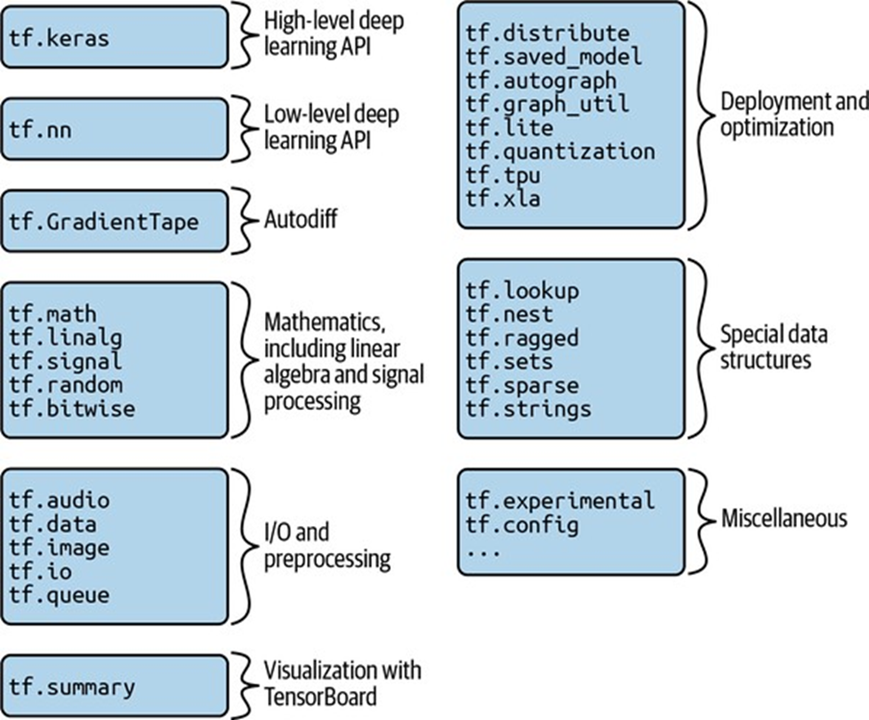
\includegraphics[width=\textwidth,height=0.7\textheight,keepaspectratio]{../machineLearningWeb/Figures/CH12/Hình_12-1}
                \vspace{0.2cm}
                \textit{Hình 12-1: Tổng quan về API Python của TensorFlow}
            \end{center}
        \end{column}
    \end{columns}
\end{frame}

\begin{frame}{Tổng quan về API Python của TensorFlow (2/2)}
    \begin{itemize}
        \item Sự trừu tượng hóa các mức độ phức tạp giúp người học mới tiếp cận qua Keras một cách nhanh chóng.
        \item Trong khi đó, các nhà nghiên cứu sâu (researchers) vẫn có thể dùng các API cấp thấp để viết các thuật toán huấn luyện phi tiêu chuẩn (như trong GANs hay Meta-learning).
        \item Hình 12-1 tóm tắt một cách bao quát các module quan trọng mà TensorFlow cung cấp.
        \item Chúng ta sẽ lần lượt khám phá từ Tensor cơ bản đến việc tùy chỉnh các lớp và mô hình thông qua API này.
    \end{itemize}
\end{frame}

\begin{frame}{Kiến trúc của TensorFlow (1/2)}
    \begin{columns}
        \begin{column}{0.4\textwidth}
            \begin{itemize}
                \item Hình 12-2 minh họa kiến trúc bên trong của TensorFlow.
                \item Lớp Execution Engine ở trung tâm thực hiện các biểu đồ (Graphs) bằng C++ (mã nguồn lõi được tối ưu cực cao).
                \item Cung cấp khả năng chạy đồng thời (multi-threading) trên nhiều loại phần cứng (CPU, GPU, TPU) và qua mạng (Android, iOS, Cloud).
            \end{itemize}
        \end{column}
        \begin{column}{0.6\textwidth}
            \begin{center}
                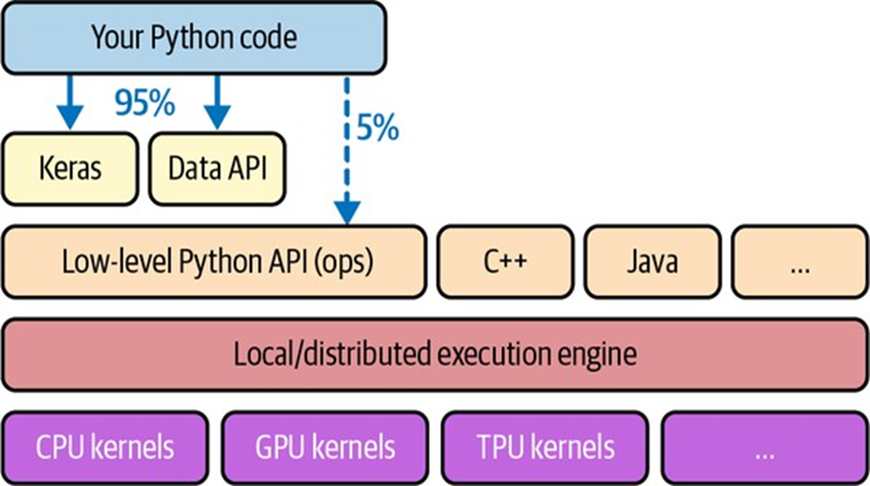
\includegraphics[width=\textwidth,height=0.7\textheight,keepaspectratio]{../machineLearningWeb/Figures/CH12/Hình_12-2}
                \vspace{0.2cm}
                \textit{Hình 12-2: Kiến trúc của TensorFlow}
            \end{center}
        \end{column}
    \end{columns}
\end{frame}

\begin{frame}{Kiến trúc của TensorFlow (2/2)}
    \begin{itemize}
        \item API giao diện bằng nhiều ngôn ngữ: Python (phổ biến nhất), C++, Java, Go, Swift.
        \item Hầu hết thời gian bạn sẽ chỉ cần tương tác qua Keras (High-level API). 
        \item Lớp \textbf{XLA (Accelerated Linear Algebra)}: Trình biên dịch mạnh mẽ, giúp tối ưu hóa thêm các Graph, kết hợp các toán tử lại (kernel fusion) nhằm tăng tốc tối đa tốc độ xử lý phần cứng.
        \item TF Distributed Execution: Trực tiếp phân phối khối lượng tính toán trên nhiều máy vật lý (Parameter Server, MirroredStrategy).
    \end{itemize}
\end{frame}

\section{Sử dụng TensorFlow như NumPy}

\begin{frame}[fragile]{Tensor và Phép toán (Tensors and Operations)}
    \begin{itemize}
        \item API của TensorFlow chủ yếu xoay quanh các \textit{tensors} (cáp số liệu đa chiều).
        \item Khái niệm Tensors được kế thừa từ Toán học, dùng để đại diện cho đại lượng vô hướng (scalar - 0D), vectơ (1D), ma trận (2D) hoặc không gian đa chiều (nD).
        \item Cách dễ nhất để tạo tensor là dùng \texttt{tf.constant()}.
    \end{itemize}
    \begin{lstlisting}[language=Python]
import tensorflow as tf

# Tao tensor tu ma tran 2 chieu (2D)
t = tf.constant([[1., 2., 3.], [4., 5., 6.]])
print(t.shape) # In ra: TensorShape([2, 3])
print(t.dtype) # In ra: <dtype: 'float32'>
    \end{lstlisting}
\end{frame}

\begin{frame}[fragile]{Các hàm toán học cơ bản}
    \begin{itemize}
        \item TensorFlow cung cấp hàng loạt hàm toán học mạnh mẽ hoạt động trực tiếp trên tensors mà không cần vòng lặp for.
        \item Các toán tử chuẩn Python (\texttt{+}, \texttt{-}, \texttt{*}, \texttt{/}, \texttt{**}) đã được nạp chồng (overloaded).
    \end{itemize}
    \begin{lstlisting}[language=Python]
# Tinh toan co ban bang TF operations
t1 = t + 10                 # Phep cong (hoat dong broadcasting)
t2 = tf.square(t)           # Binh phuong tung phan tu (element-wise)
t3 = t @ tf.transpose(t)    # Nhan ma tran (Matrix multiplication)
    \end{lstlisting}
    \begin{itemize}
        \item Ký hiệu \texttt{@} xuất hiện từ Python 3.5 để thay thế cho phép nhân ma trận (\texttt{tf.matmul}).
        \item Các hàm phổ biến khác: \texttt{tf.exp()}, \texttt{tf.sqrt()}, \texttt{tf.reduce\_sum()}, \texttt{tf.reduce\_mean()}.
    \end{itemize}
\end{frame}

\begin{frame}[fragile]{Tensors và NumPy: Tương tác qua lại}
    \begin{itemize}
        \item Tensors tương tác rất thân thiện và liền mạch với thư viện NumPy - tiêu chuẩn của khoa học dữ liệu.
        \item Có thể tạo tensor trực tiếp từ một mảng NumPy, và ngược lại.
    \end{itemize}
    \begin{lstlisting}[language=Python]
import numpy as np

# Chuyen Numpy -> Tensor
a = np.array([2., 4., 5.])
t_a = tf.constant(a)

# Chuyen Tensor -> Numpy
a_back = t_a.numpy()        # Ban co thu dung np.array(t_a)

# Tinh toan ket hop (Cross-computation)
t_b = tf.square(a)          # TF chap nhan Numpy array 
a_b = np.square(t_a)        # Numpy chap nhan TF Tensor 
    \end{lstlisting}
\end{frame}

\begin{frame}[fragile]{Lưu ý khi dùng chung Numpy và TensorFlow}
    \begin{itemize}
        \item Mặc dù chúng có thể được truyền vào hàm của nhau, nhưng bạn nên ưu tiên dùng hàm TensorFlow nếu muốn tận dụng tốc độ của GPU.
        \item NumPy chỉ chạy được duy nhất trên CPU. Nếu một Tensor đang nằm trên GPU mà bạn gọi hàm NumPy, TensorFlow sẽ phải \textbf{sao chép dữ liệu từ bộ nhớ GPU về CPU} $\rightarrow$ Chi phí truyền tải lớn.
        \item Khác biệt nhỏ về kiểu dữ liệu: NumPy mặc định dùng float64 cho độ chính xác cao. TensorFlow mặc định dùng float32 (thậm chí bfloat16) vì mạng Neural quan trọng tính hiệu suất.
    \end{itemize}
\end{frame}

\begin{frame}[fragile]{Chuyển đổi kiểu dữ liệu (Type Conversions)}
    \begin{itemize}
        \item TensorFlow \textbf{không tự động} ép kiểu (type conversion) giống như Python hay NumPy.
        \item Việc thực hiện ép kiểu giữa \texttt{float32} và \texttt{float64} hoặc \texttt{float32} và \texttt{int32} có chi phí tính toán cao.
    \end{itemize}
    \begin{lstlisting}[language=Python]
# Kieu int32 khong the cong voi float32 ngam dinh:
# tf.constant(2.0) + tf.constant(40) # --> Loi TypeError

# Can phai ep kieu chu dong va ro rang bang tf.cast:
t2 = tf.constant(40., dtype=tf.float64)

# tf.cast(t2, tf.float32) ha do chinh xac xuong float32
result = tf.constant(2.0) + tf.cast(t2, tf.float32)
    \end{lstlisting}
\end{frame}

\begin{frame}[fragile]{Biến số (Variables)}
    \begin{itemize}
        \item Đặc tính của \texttt{tf.constant()} là không thể thay đổi (immutable). Ta không thể gán lại một giá trị cho một phần tử bên trong nó.
        \item Tuy nhiên, mạng nơ-ron liên tục cập nhật \textbf{trọng số (weights)} và độ lệch (biases) qua mỗi chu kỳ học (epoch). 
        \item Do đó, ta cần sử dụng cấu trúc \texttt{tf.Variable}.
    \end{itemize}
    \begin{lstlisting}[language=Python]
v = tf.Variable([[1., 2., 3.], [4., 5., 6.]])

# Cap nhat toan bo bien (dung phuong thuc assign)
v.assign(2 * v)

# Cap nhat vao dung 1 vi tri cu the (nhu numpy arrays)
v[0, 1].assign(42)

# Cap nhat toan cuc bang phep cong (+), tru (-)
v.assign_add([[1., 1., 1.], [1., 1., 1.]])
    \end{lstlisting}
\end{frame}

\begin{frame}{Các cấu trúc dữ liệu nâng cao khác}
    \begin{itemize}
        \item \textbf{Sparse tensors (\texttt{tf.SparseTensor}):} Tối ưu bộ nhớ cho ma trận chứa phần lớn giá trị là 0. Lưu trữ 3 mảng: \textit{indices}, \textit{values}, \textit{dense\_shape}.
        \item \textbf{Tensor arrays (\texttt{tf.TensorArray}):} Một danh sách các Tensors cho phép append động. Rất hữu ích cho các mạng tuần tự RNN.
        \item \textbf{Ragged tensors (\texttt{tf.RaggedTensor}):} Đại diện mảng bất đối xứng. VD: danh sách chứa các chuỗi con có độ dài không bằng nhau.
        \item \textbf{String tensors:} Tensor lưu trữ kiểu chữ (strings), các chuỗi ký tự UTF-8 hoặc byte arrays, cần thiết cho NLP.
        \item \textbf{Sets:} Tập hợp Toán học dưới dạng Sparse tensor bằng \texttt{tf.sets}.
    \end{itemize}
\end{frame}

\section{Tùy chỉnh mô hình và Thành phần (Custom Components)}

\begin{frame}{Tại sao cần tùy chỉnh mô hình trong Keras?}
    \begin{itemize}
        \item Keras API cung cấp sẵn hàng chục hàm \textit{losses, metrics, layers, optimizers} chuẩn mực. Đa số bài toán chỉ cần gọi tên chuỗi, ví dụ: \texttt{loss="mse"}, \texttt{activation="relu"}.
        \item \textbf{Thực tế phức tạp hơn:}
        \begin{enumerate}
            \item Bài toán đặc thù yêu cầu hàm tính sai số hoàn toàn mới: Phạt lỗi sai số dương nặng gấp đôi sai số âm.
            \item Nghiên cứu tạo ra một cấu trúc Tầng Nơ-ron (Layer) chưa từng có.
            \item Xây dựng mạng với 3 nguồn dữ liệu vào (Multi-input) và 2 luồng kết quả xuất ra (Multi-output).
        \end{enumerate}
        \item TensorFlow 2 cho phép dùng Python viết mọi thứ, đóng gói lại và dùng như Module nguyên bản.
    \end{itemize}
\end{frame}

\begin{frame}[fragile]{Tùy chỉnh Hàm mất mát (Custom Loss) - Huber Loss (1/2)}
    \begin{itemize}
        \item Ví dụ bài toán dự đoán giá cả. Lỗi (error = label - prediction). 
        \item Mean Squared Error (MSE) phạt bình phương lỗi, rất nhạy cảm nhiễu. Mean Absolute Error (MAE) trừng phạt tuyến tính, nhưng không mượt quanh điểm 0.
        \item \textbf{Huber Loss:} Hành vi giống MSE khi lỗi nhỏ, giống MAE khi lỗi lớn. 
    \end{itemize}
    \begin{lstlisting}[language=Python]
def huber_fn(y_true, y_pred):
    error = y_true - y_pred
    is_small_error = tf.abs(error) < 1
    squared_loss = tf.square(error) / 2
    linear_loss  = tf.abs(error) - 0.5
    # Dung tf.where() giong nhu np.where()
    return tf.where(is_small_error, squared_loss, linear_loss)
    \end{lstlisting}
\end{frame}

\begin{frame}[fragile]{Tùy chỉnh Hàm mất mát (Custom Loss) - Sử dụng (2/2)}
    \begin{itemize}
        \item Dùng hàm Python trực tiếp vào tham số \texttt{loss} khi biên dịch mô hình.
    \end{itemize}
    \begin{lstlisting}[language=Python]
# Truyen truc tiep ten ham huber vao phuong thuc compile
model.compile(loss=huber_fn, optimizer="nadam", metrics=["mae"])

# Huan luyen nhu binh thuong
model.fit(X_train, y_train, epochs=2)
    \end{lstlisting}
    \begin{itemize}
        \item Keras sẽ truyền \texttt{y\_true} và \texttt{y\_pred} (Tensor) vào \texttt{huber\_fn} tự động trong mỗi batch, tính sai số, rồi tự động truy vết lại để tính đạo hàm cập nhật ngược.
    \end{itemize}
\end{frame}

\begin{frame}[fragile]{Lưu ý khi tải (load) mô hình chứa Custom Loss}
    \begin{itemize}
        \item Cấu trúc Keras không lưu trữ mã nguồn Python của hàm \texttt{huber\_fn}.
        \item \textbf{Vấn đề:} Khi dùng \texttt{keras.models.load\_model()} ở script khác, Keras sẽ báo lỗi "Unknown loss function".
    \end{itemize}
    \begin{lstlisting}[language=Python]
# Luu nhu binh thuong
model.save("my_model_with_a_custom_loss.h5")

# Khi load, ban BAT BUOC phai truyen tu dien (dictionary) 
# khai bao mapping tu chuoi sang doi tuong Python
model = keras.models.load_model(
    "my_model_with_a_custom_loss.h5",
    custom_objects={"huber_fn": huber_fn}
)
    \end{lstlisting}
\end{frame}

\begin{frame}[fragile]{Xây dựng Custom Loss bằng OOP (Subclassing) (1/2)}
    \begin{itemize}
        \item Nếu hàm Loss yêu cầu siêu tham số (như \texttt{threshold=1.0} không cố định), sử dụng Hàm Python rất bất tiện.
        \item Giải pháp OOP: Kế thừa lớp \texttt{keras.losses.Loss}. Khai báo \texttt{get\_config()} để tự động lưu tham số.
    \end{itemize}
    \begin{lstlisting}[language=Python]
class HuberLoss(keras.losses.Loss):
    def __init__(self, threshold=1.0, **kwargs):
        self.threshold = threshold
        super().__init__(**kwargs)
        
    def call(self, y_true, y_pred):
        error = y_true - y_pred
        is_small_error = tf.abs(error) < self.threshold
        squared_loss = tf.square(error) / 2
        linear_loss  = self.threshold * tf.abs(error) - self.threshold**2 / 2
        return tf.where(is_small_error, squared_loss, linear_loss)
    \end{lstlisting}
\end{frame}

\begin{frame}[fragile]{Xây dựng Custom Loss bằng OOP (Subclassing) (2/2)}
    \begin{itemize}
        \item Cung cấp \texttt{get\_config()} để lưu trữ tham số mạnh mẽ hơn. 
    \end{itemize}
    \begin{lstlisting}[language=Python]
    def get_config(self):
        base_config = super().get_config()
        # Cap nhat thong so cua minh kem theo thong so cha
        return {**base_config, "threshold": self.threshold}

# Chi can tao doi tuong thay vi day string
model.compile(loss=HuberLoss(2.), optimizer="nadam")

# Keras goi get_config de luu threshold=2. vao JSON Model.
model.save("my_custom_model_v2.h5")

# Khi load, custom_objects van la bat buoc!
model = keras.models.load_model("my_custom_model_v2.h5", 
        custom_objects={"HuberLoss": HuberLoss})
    \end{lstlisting}
\end{frame}

\begin{frame}[fragile]{Tùy chỉnh Hàm Đánh giá (Custom Metrics)}
    \begin{itemize}
        \item Bạn có thể tái sử dụng Custom Loss cho Metric. Loss dùng để huấn luyện, Metric in ra để đánh giá.
    \end{itemize}
    \begin{lstlisting}[language=Python]
model.compile(loss="mse", optimizer="nadam", 
              metrics=[huber_fn])
    \end{lstlisting}
    \begin{itemize}
        \item \textbf{Vấn đề:} Metrics tiêu chuẩn Keras là "Streaming metrics", tính luỹ kế qua các batch rồi chia trung bình. Hàm Python đơn giản sẽ bị tính sai luỹ kế.
        \item Giải pháp nâng cao là kế thừa \texttt{keras.metrics.Metric}, quản lý các biến trạng thái bằng \texttt{self.add\_weight()} và ghi đè hàm \texttt{update\_state()}, \texttt{result()}.
    \end{itemize}
\end{frame}

\begin{frame}[fragile]{Tùy chỉnh Lớp ẩn không trạng thái (Stateless Custom Layers)}
    \begin{itemize}
        \item Nếu cấu trúc phi tuyến đặc biệt không chứa tham số cấu hình cần học (Weights/Biases), Keras cung cấp \texttt{keras.layers.Lambda}.
    \end{itemize}
    \begin{lstlisting}[language=Python]
# Tao tang mu (exponential layer)
exponential_layer = keras.layers.Lambda(lambda x: tf.exp(x))

# Tich hop vao Sequential Model
model = keras.models.Sequential([
    keras.layers.Dense(30, activation="relu"),
    keras.layers.Dense(1),
    exponential_layer
])
    \end{lstlisting}
    \begin{itemize}
        \item Layer kiểu này có thể đóng vai trò làm activation function hoặc preprocessing.
    \end{itemize}
\end{frame}

\begin{frame}[fragile]{Tùy chỉnh Lớp ẩn có trạng thái (Stateful Custom Layer) (1/2)}
    \begin{itemize}
        \item Để tạo Layer riêng có khả năng "Học" hệ số $W, b$, bạn kế thừa \texttt{keras.layers.Layer}.
        \item Gồm 3 hàm: \texttt{\_\_init\_\_}, \texttt{build()} (khởi tạo Weights khi nhận dạng Shape) và \texttt{call()} (thực thi Feed-Forward).
    \end{itemize}
    \begin{lstlisting}[language=Python]
class MyDense(keras.layers.Layer):
    def __init__(self, units, activation=None, **kwargs):
        super().__init__(**kwargs)
        self.units = units
        self.activation = keras.activations.get(activation)

    def build(self, batch_input_shape):
        self.kernel = self.add_weight(
            name="kernel", shape=[batch_input_shape[-1], self.units],
            initializer="glorot_normal")
    \end{lstlisting}
\end{frame}

\begin{frame}[fragile]{Tùy chỉnh Lớp ẩn có trạng thái (Stateful Custom Layer) (2/2)}
    \begin{lstlisting}[language=Python]
        # Tiep tuc ham build
        self.bias = self.add_weight(
            name="bias", shape=[self.units], initializer="zeros")
        super().build(batch_input_shape) 

    def call(self, X):
        return self.activation(X @ self.kernel + self.bias)

    def compute_output_shape(self, batch_input_shape):
        return tf.TensorShape(batch_input_shape.as_list()[:-1] + [self.units])
    \end{lstlisting}
    \begin{itemize}
        \item Bằng cách này, Layer tùy biến có thể nối chuỗi trong \texttt{Sequential} một cách trong suốt.
    \end{itemize}
\end{frame}

\begin{frame}{Tùy chỉnh toàn bộ Mô hình (Custom Models)}
    \begin{itemize}
        \item Khi xây dựng kiến trúc không dạng tuần tự (VD: mạng lưới có đường chéo, Residual Neural Networks), \texttt{Sequential} trở nên cồng kềnh.
        \item \textbf{Phương pháp Model Subclassing:} Cho phép ta thiết kế bằng Python tự do: Có thể dùng \texttt{if...else} luồng điều hướng, vòng lặp \texttt{for} để nối module động.
        \item Ta sẽ trình bày mô hình mẫu sử dụng một lớp khối (Residual Block) với khả năng \textit{Skip Connection}.
    \end{itemize}
\end{frame}

\begin{frame}{Mô hình tùy chỉnh: Residual Block}
    \begin{columns}
        \begin{column}{0.4\textwidth}
            \begin{itemize}
                \item Hình 12-3 phác thảo cấu trúc một kiến trúc tùy ý với kỹ thuật \textbf{Skip connection}.
                \item Đường đi thẳng truyền trực tiếp Input cộng với Output của chuỗi tầng ẩn.
                \item Giải quyết triệt để lỗi mất gradient (Vanishing Gradient) trong Deep Learning.
            \end{itemize}
        \end{column}
        \begin{column}{0.6\textwidth}
            \begin{center}
                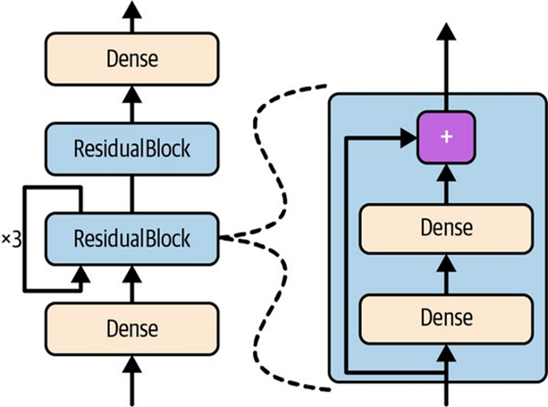
\includegraphics[width=\textwidth,height=0.7\textheight,keepaspectratio]{../machineLearningWeb/Figures/CH12/Hình_12-3}
                \vspace{0.2cm}
                \textit{Hình 12-3: Ví dụ mô hình tùy chỉnh: một mô hình tùy ý với lớp ResidualBlock tùy chỉnh chứa kết nối}
            \end{center}
        \end{column}
    \end{columns}
\end{frame}

\begin{frame}[fragile]{Mã Python Xây dựng Residual Block}
    \begin{itemize}
        \item Viết một Custom Layer đóng vai trò chứa chuỗi \texttt{Dense} và làm phép tính \texttt{+} kết nối.
    \end{itemize}
    \begin{lstlisting}[language=Python]
class ResidualBlock(keras.layers.Layer):
    def __init__(self, n_layers, n_neurons, **kwargs):
        super().__init__(**kwargs)
        self.hidden = [keras.layers.Dense(n_neurons, activation="elu")
                       for _ in range(n_layers)]
                       
    def call(self, inputs):
        Z = inputs
        # Vong lap for feed-forward
        for layer in self.hidden:
            Z = layer(Z)
        # Phep Cong Skip Connection
        return inputs + Z
    \end{lstlisting}
\end{frame}

\begin{frame}[fragile]{Xây dựng Custom Model sử dụng Residual Block}
    \begin{itemize}
        \item Kế thừa \texttt{keras.Model} giống kế thừa Layer, cấu trúc \texttt{\_\_init\_\_} và \texttt{call()} tương tự.
    \end{itemize}
    \begin{lstlisting}[language=Python]
class ResidualRegressor(keras.Model):
    def __init__(self, output_dim, **kwargs):
        super().__init__(**kwargs)
        self.hidden1 = keras.layers.Dense(30, activation="elu")
        self.block1 = ResidualBlock(2, 30)
        self.block2 = ResidualBlock(2, 30)
        self.out = keras.layers.Dense(output_dim)

    def call(self, inputs):
        Z = self.hidden1(inputs)
        for _ in range(1 + 3): # 4 lan di qua Block 1
            Z = self.block1(Z)
        Z = self.block2(Z)     # 1 lan di qua Block 2
        return self.out(Z)
    \end{lstlisting}
\end{frame}

\begin{frame}{Model Subclassing vs Functional API}
    \begin{itemize}
        \item \textbf{Subclassing API} cung cấp sự linh hoạt cực lớn (dùng vòng \texttt{for}, luồng logic động). 
        \item Tuy nhiên, nhược điểm chí mạng là Keras \textbf{không thể lưu đồ thị} \texttt{model.summary()} hoặc vẽ \texttt{plot\_model()} khi chưa truyền thử bộ dữ liệu (\textit{Model is not Built}). 
        \item Lỗi logic luồng xử lý bên trong Python rất khó phát hiện.
        \item \textbf{Lời khuyên:} Hãy dùng Functional API nếu có thể, trừ phi mạng có vòng lặp động hoặc điều kiện tùy thuộc dữ liệu sinh ra (dynamic branching).
    \end{itemize}
\end{frame}

\section{Hàm và biểu đồ TensorFlow (AutoGraph)}

\begin{frame}{Chế độ Tức thời (Eager) vs Chế độ Biểu đồ (Graph)}
    \begin{itemize}
        \item TensorFlow 1.x yêu cầu định nghĩa đồ thị trước, rồi mở \texttt{tf.Session} để thực thi (Graph Execution). Quá trình debug vô cùng tàn bạo.
        \item TensorFlow 2.x đổi phương thức hoạt động mặc định thành \textbf{Eager Execution} - Chế độ thực thi tức thì.
        \item Mã chạy dòng nào có kết quả ngay. Gỡ lỗi bằng \texttt{print()} truyền thống.
        \item \textbf{Khuyết điểm:} Eager Mode Chậm hơn nhiều so với Graph (không thể tối ưu song song hóa phần cứng).
    \end{itemize}
\end{frame}

\begin{frame}[fragile]{\texttt{@tf.function}: Phép màu của AutoGraph}
    \begin{itemize}
        \item TensorFlow 2 mang đến giải pháp dung hòa bằng AutoGraph!
        \item Bạn viết code Python bình thường, chỉ cần đánh dấu \texttt{@tf.function}. TF sẽ tự động dịch thành đồ thị C++ ẩn bên dưới.
    \end{itemize}
    \begin{lstlisting}[language=Python]
def cube(x):
    return x ** 3

# Tinh toan - Nhanh cho Test nhung cham khi huan luyen
cube(tf.constant(2.0))

# Khai bao TF Function bang decorator
@tf.function
def tf_cube(x):
    return x ** 3

# tf_cube tro thanh mot computational graph!
tf_cube(tf.constant(2.0)) 
    \end{lstlisting}
\end{frame}

\begin{frame}{Cách AutoGraph tạo Biểu đồ và Tracing (1/2)}
    \begin{columns}
        \begin{column}{0.4\textwidth}
            \begin{itemize}
                \item Hình 12-4 mô tả cơ chế của AutoGraph.
                \item Mã Python được quét, tạo Abstract Syntax Tree.
                \item Sinh ra hàm Python nâng cấp gọi các toán tử điều khiển lõi của TF như \texttt{tf.cond}, \texttt{tf.while\_loop}.
            \end{itemize}
        \end{column}
        \begin{column}{0.6\textwidth}
            \begin{center}
                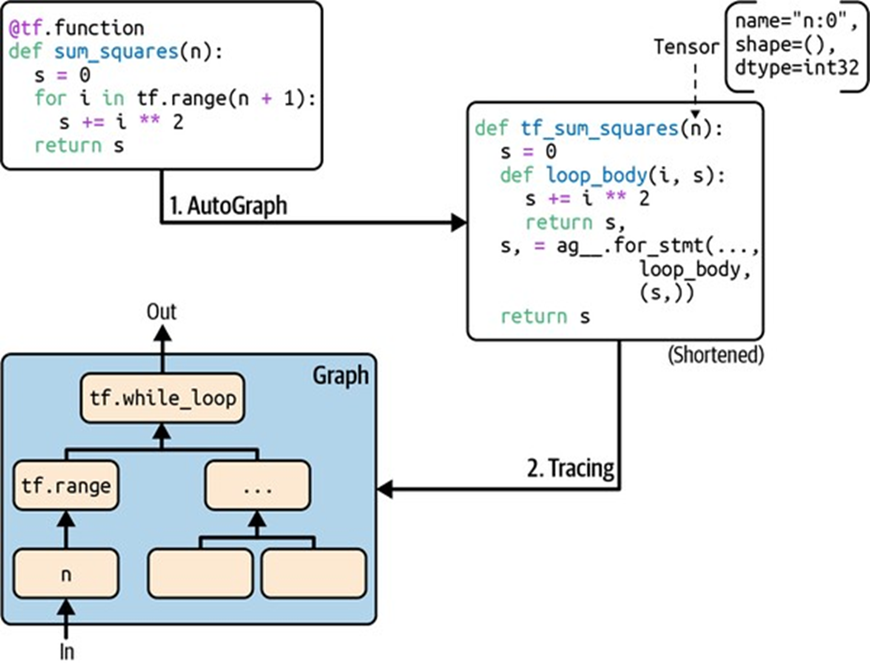
\includegraphics[width=\textwidth,height=0.7\textheight,keepaspectratio]{../machineLearningWeb/Figures/CH12/Hình_12-4}
                \vspace{0.2cm}
                \textit{Hình 12-4: Cách TensorFlow tạo biểu đồ bằng AutoGraph và tracing}
            \end{center}
        \end{column}
    \end{columns}
\end{frame}

\begin{frame}{Cách AutoGraph tạo Biểu đồ và Tracing (2/2)}
    \begin{itemize}
        \item Khi thực thi lần đầu tiên (\textbf{Tracing}), nó vạch ra lộ trình các phép toán thành \textbf{TensorFlow Graph}.
        \item Lần thực thi tiếp theo chạy Graph trực tiếp.
        \item Chú ý: TensorFlow tạo Poly-morphism (Đa hình đồ thị). Nếu gọi Input \texttt{int32}, nó tạo Graph 1. Nếu gọi \texttt{float32}, lưu thêm Graph 2.
    \end{itemize}
\end{frame}

\begin{frame}[fragile]{Giới hạn và Quy tắc sống còn của TF Functions (1/2)}
    \begin{itemize}
        \item \textbf{Side effects:} Hàm \texttt{print()} hoặc thao tác IO \textbf{chỉ chạy một lần duy nhất} ở giai đoạn Tracing, không nằm trong Đồ thị.
    \end{itemize}
    \begin{lstlisting}[language=Python]
@tf.function
def my_func(x):
    print("Ham dang duoc trace:", x.dtype)
    return x + 1

my_func(tf.constant(1.0)) # In log, Tao Graph float32
my_func(tf.constant(2.0)) # KHONG in log, Tai su dung Graph float32
my_func(tf.constant(10))  # In log, Tao Graph int32
    \end{lstlisting}
    \begin{itemize}
        \item Muốn in log động? Sử dụng \texttt{tf.print()}.
    \end{itemize}
\end{frame}

\begin{frame}[fragile]{Giới hạn và Quy tắc sống còn của TF Functions (2/2)}
    \begin{itemize}
        \item \textbf{Biến ngoài hàm / List Python:} Nếu dùng \texttt{list.append()}, list bị "đóng băng" ở trace. Hãy dùng \texttt{tf.TensorArray}.
        \item Tránh sinh số ngẫu nhiên bằng Numpy (\texttt{np.random.rand()}), hãy sử dụng \texttt{tf.random}.
    \end{itemize}
    \begin{lstlisting}[language=Python]
@tf.function
def add_random_noise(x):
    # SAI LAM: Gia tri ngau nhien bi dong bang
    # noise = np.random.randn()  
    
    # CHUAN XAC: Gia tri ngau nhien sinh ra moi khi goi Graph
    noise = tf.random.normal(shape=[])
    return x + noise
    \end{lstlisting}
\end{frame}

\section{Vòng lặp Huấn luyện Tùy chỉnh}

\begin{frame}{Vòng lặp huấn luyện tùy chỉnh}
    \begin{itemize}
        \item Phương thức \texttt{model.fit()} tiện lợi, nhưng không phải kiến trúc nào cũng xài được (VD: mạng GAN huấn luyện Generator 1 bước, Discriminator 1 bước).
        \item Viết vòng lặp tùy chỉnh (Custom Training Loop) mất công, nhưng cho phép tùy biến không giới hạn.
    \end{itemize}
\end{frame}

\begin{frame}[fragile]{\texttt{tf.GradientTape()}: Tính đạo hàm tự động}
    \begin{itemize}
        \item TensorFlow cung cấp \texttt{GradientTape} đóng vai trò "băng ghi âm" lưu vết Tensor để lan truyền ngược (Backpropagation) tính đạo hàm tự động.
    \end{itemize}
    \begin{lstlisting}[language=Python]
def f(w1, w2):
    return 3 * w1 ** 2 + 2 * w1 * w2

w1, w2 = tf.Variable(5.), tf.Variable(3.)

with tf.GradientTape() as tape:
    z = f(w1, w2)

# Yeu cau Tape tinh dao ham Z theo bien w1, w2
gradients = tape.gradient(z, [w1, w2])
print(gradients) 
# Ket qua: dz/dw1=36, dz/dw2=10
    \end{lstlisting}
\end{frame}

\begin{frame}[fragile]{GradientTape nâng cao}
    \begin{itemize}
        \item Mặc định, `GradientTape` chỉ theo dõi biến `tf.Variable`. Không theo dõi `tf.constant`.
        \item Khi gọi phương thức `gradient()`, bộ nhớ Tape bị xóa.
        \item Tính nhiều lần đạo hàm (VD: Hessian), dùng cờ `persistent=True`.
    \end{itemize}
    \begin{lstlisting}[language=Python]
with tf.GradientTape(persistent=True) as tape:
    z = f(w1, w2)

dz_dw1 = tape.gradient(z, w1)
dz_dw2 = tape.gradient(z, w2)  # Van OK

# Giai phong bo nho bang tay (bat buoc)
del tape
    \end{lstlisting}
\end{frame}

\begin{frame}[fragile]{Viết Vòng lặp huấn luyện - Khởi tạo}
    \begin{itemize}
        \item Tạo mô hình, cấu hình siêu tham số, Optimizer, Metric và Dữ liệu.
    \end{itemize}
    \begin{lstlisting}[language=Python]
l2_reg = keras.regularizers.l2(0.05)
model = keras.models.Sequential([
    keras.layers.Dense(30, activation="elu", kernel_regularizer=l2_reg),
    keras.layers.Dense(1, kernel_regularizer=l2_reg)
])

batch_size = 32
train_set = tf.data.Dataset.from_tensor_slices((X_train, y_train))
train_set = train_set.shuffle(len(X_train)).batch(batch_size)

optimizer = keras.optimizers.Nadam(learning_rate=0.01)
loss_fn = keras.losses.mean_squared_error
mean_loss = keras.metrics.Mean() 
    \end{lstlisting}
\end{frame}

\begin{frame}[fragile]{Viết Vòng lặp huấn luyện - Thực thi (Epochs \& Steps)}
    \begin{itemize}
        \item Lặp qua Epochs, trong Epochs lặp qua DataBatches.
    \end{itemize}
    \begin{lstlisting}[language=Python]
epochs = 5
for epoch in range(epochs):
    for step, (X_batch, y_batch) in enumerate(train_set):
        
        # 1. Forward pass ghi bang Tape
        with tf.GradientTape() as tape:
            y_pred = model(X_batch, training=True) 
            main_loss = tf.reduce_mean(loss_fn(y_batch, y_pred))
            loss = tf.add_n([main_loss] + model.losses)
            
        # 2. Tinh Gradient theo model variables
        gradients = tape.gradient(loss, model.trainable_variables)
        
        # 3. Kich hoat phuong thuc cap nhat trong so (Optimize)
        optimizer.apply_gradients(zip(gradients, model.trainable_variables))
    \end{lstlisting}
\end{frame}

\begin{frame}{Cấu trúc hoàn chỉnh và Những lưu ý quan trọng}
    \begin{itemize}
        \item Bạn phải chịu trách nhiệm đảm bảo mọi thứ chính xác:
        \begin{enumerate}
            \item Truyền cờ \texttt{training=True} vào lệnh dự đoán của model để \textit{BatchNormalization}/\textit{Dropout} hoạt động đúng.
            \item Theo dõi Metric thủ công (\texttt{update\_state(loss)}), in ra cuối Epoch và gọi \texttt{reset\_states()}.
            \item Xử lý cập nhật biến hệ thống (Non-trainable variables, như trung bình trượt của Batch Norm).
        \end{enumerate}
    \end{itemize}
\end{frame}

\begin{frame}[fragile]{Tối ưu hóa Vòng lặp với @tf.function}
    \begin{itemize}
        \item Vòng lặp \texttt{for} Python qua DataBatches siêu chậm.
        \item Lời khuyên: Đóng gói quá trình xử lý 1 Bước (1 Step) thành \texttt{@tf.function} để tăng tốc biên dịch toán học C++.
    \end{itemize}
    \begin{lstlisting}[language=Python]
@tf.function
def train_step(X_batch, y_batch):
    with tf.GradientTape() as tape:
        y_pred = model(X_batch, training=True)
        main_loss = tf.reduce_mean(loss_fn(y_batch, y_pred))
        loss = tf.add_n([main_loss] + model.losses)
    gradients = tape.gradient(loss, model.trainable_variables)
    optimizer.apply_gradients(zip(gradients, model.trainable_variables))

# Trong vong lap chi goi train_step(X_batch, y_batch)
    \end{lstlisting}
\end{frame}

\begin{frame}{Tóm tắt}
    \begin{itemize}
        \item \textbf{Cốt lõi TensorFlow} đại lượng Tensors cực kỳ giống NumPy, tối ưu đa phần cứng (GPU/TPU).
        \item Việc \textbf{tùy biến Keras (Custom Component)} cho phép người học và nghiên cứu làm mới hoàn toàn Losses, Metrics, Layers, Models.
        \item \textbf{AutoGraph (\texttt{@tf.function})} giải quyết sự tranh chấp linh hoạt kịch bản (Python) với biên dịch nhanh chóng.
        \item \textbf{\texttt{tf.GradientTape}} đưa quyền kiểm soát hoàn toàn tới luồng huấn luyện cho các nghiên cứu mới.
    \end{itemize}
\end{frame}

\end{document}
